\chapter{网络流应用}

\begin{introduction}
	\item 最大二分匹配问题
	\item Tiling Problem
	\item 棒球比赛
	\item 项目选择
\end{introduction}

本章是在基于网络流FF算法的基础上,学习网络流的应用。

\section{最大二分匹配问题}

\begin{definition}{二分图}{bipartite-graph}
	对于无向图\(G = (V,\,E)\),若顶点集V可以分割为两个互不相交子集\((X,\,Y)\),使得边集\(E\)中任意一条边\(e = (u,\,v)\),都可以满足\(u \in X\) ,\(v \in Y\),则称图\(G\)为二分图。
\end{definition}

问题: 对于给定的\(G = (V,\,E)\),\(V\)为\(V_l \cup V_r\),\(V_l \cap V_r = \phi \),找到\(V_l\)到\(V_r\)的最大匹配。

\begin{definition}{匹配}{matching}
	一边集M为边集E的子集,且M中任意两条边无公用顶点(不相交),则称M为图G的一个匹配。
\end{definition}

% TODO(translate): how to translate 极大匹配?
\begin{definition}{极大匹配}{great-matching}
	不是其他任何匹配的子集的匹配。
\end{definition}

\begin{definition}{最大匹配}{maximal-matching}
	极大匹配中包含最多边数的一个匹配称为最大匹配。
\end{definition}

\begin{figure}[htb]
	\centering
	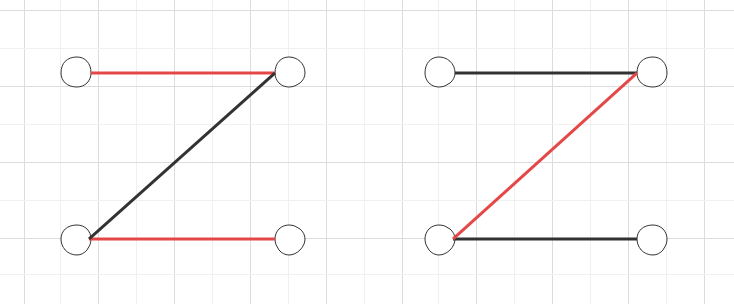
\includegraphics[scale=0.6]{image/networkflow1.png}
	\caption{极大匹配举例}\label{fig:networkflow-example1}
\end{figure}
如\autoref{fig:networkflow-example1}所示,二者都为极大匹配,但是只有左图为最大匹配。

\begin{figure}[htb]
	\centering
	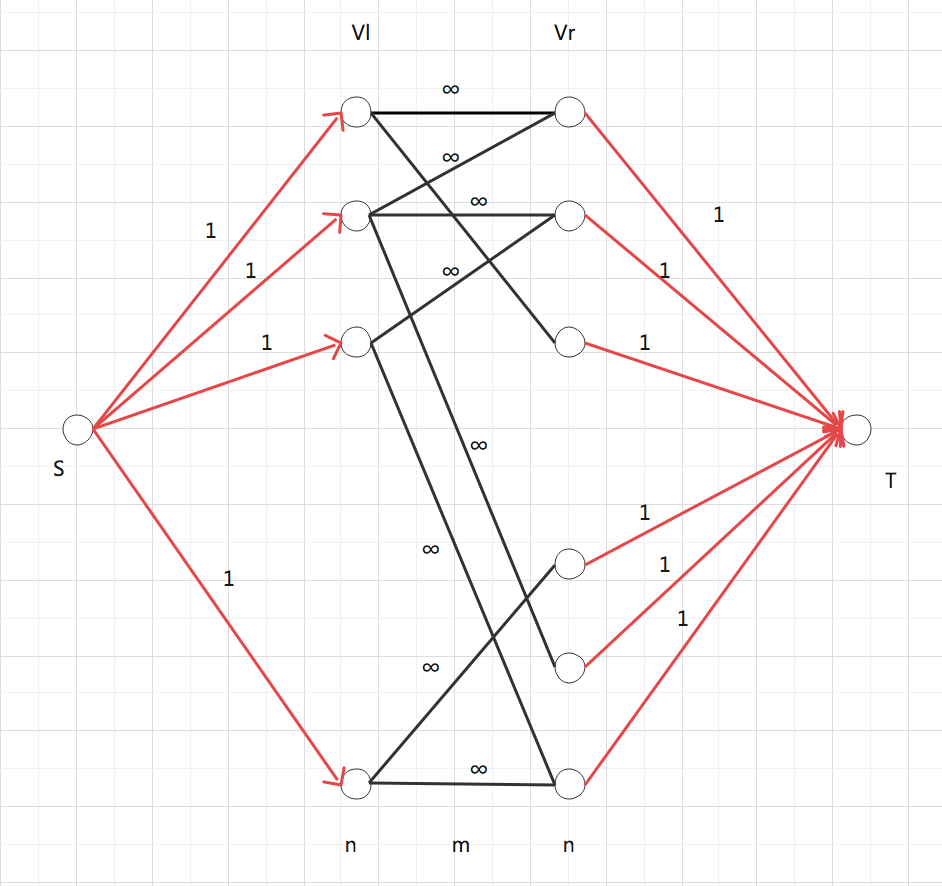
\includegraphics[scale=0.6]{image/networkflow2.png}
	\caption{FF算法建模}\label{fig:networkflow-ff-alg}
\end{figure}

使用如\autoref{fig:networkflow-ff-alg}的方法构建网络流,之后使用FF算法求解。

网络流解决最大二分匹配问题的时间复杂度为:\(O(mn)\)。

\begin{theorem}{最大流最小割定理}{max-flow-min-cut}
	指在一个网络流中,能够从源点到达汇点的最大流量等于如果从网络中移除就能够导致网络流中断的边的集合(对割的另一种理解)的最小容量和。即在任何网络中,最大流的值等于最小割的容量。
\end{theorem}

使用下面一个例子说明该算法的正确性:
\begin{figure}[htb]
	\centering
	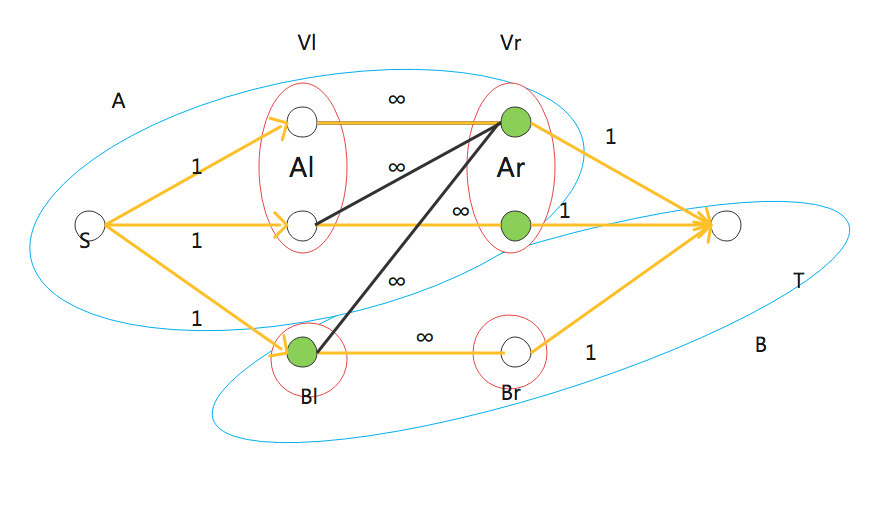
\includegraphics[scale=0.6]{image/networkflow3.png}
	\caption{算法正确性说明}\label{fig:networkflow-alg-correctness}
\end{figure}

\begin{example}
	如\autoref{fig:networkflow-alg-correctness}所示,给定二分图中,点被分为了\(V_l\)和\(V_r\)两个部分,构造网络流算法,设置一个起点S,且令S到所有的\(V_l\)中的点均有路径,容量为1;设置一个终点T,且从\(V_r\)中的点到T均有路径,容量为1。同时,所有\(V_l\)与\(V_r\)之间的路径容量均设为无穷大,由此可以找到该网络流的最大流和最小割。
\end{example}

\begin{itemize}
	\item 因为最大流等价于最小割,对于残差图Gf,从S点可以到达的点构成集合A,其他点构成集合B。
	\item 因为该图为二分图,所以不存在从\(A_l\)到\(B_l\)的路径,同样的,也不存在从\(A_r\)到\(B_r\)的路径。
	\item 因为找到了最小割,而且最小割是有限数,因此不存在从\(A_l\)到\(B_r\)的路径(已知\(A_l\)到\(B_r\)的边的容量为正无穷)。
	\item 最小割值 \(C(A,B) =|B_l|\)(实际为S流入\(B_l\)) + |\(A_r\)| (实际为 \(A_r\)流入T) = 最大流 = 最大匹配。
\end{itemize}
对于二分图来说 |最大匹配|=|最小顶点覆盖|。

\begin{definition}{完美匹配}{perfect-matching}
	所有的点均被匹配,不存在未被匹配的点。
\end{definition}

\begin{definition}{T (A)}{}
	\(A \subseteq V_l\),\(T(A) = \{b \in Vr | (a,b) \in E \} \)。
\end{definition}

对于一个二分图来说,如果\(|V_l|=|V_r|=n\),并且存在完美匹配,那么任取集合\(A \subseteq V_l,\,|T(A)| \ge |A|\)。

\begin{theorem}{霍尔定理}{hall}
	任取\(A \subseteq V_l\),若\(|T(A)| \ge |A|\),则存在完美匹配。
\end{theorem}
证明霍尔定理的正确性~(证明其逆否命题正确):
\begin{itemize}
	\item 逆否命题:若不存在完美匹配,则存在集合A,\(|T(A)| < |A|\)。
	\item \(|V_l|=|V_r|=n\),所以最大匹配\(k<n\)。
	\item 找到A,B(即S-T割),\(C(A,B) = f(A,B) = k<n\)。
	\item \(|A_l|+|B_l| = n,\,|B_l|+|A_r| = k < n\)。由此可以推出\(|A_l| > |A_r|\),可以推出\(|T(A_l)| < |A|\)。
	\item 因此,逆否命题成立,霍尔定理得证。
\end{itemize}

\section{骨牌问题}\label{sec:network-flows-tiling}
回顾本课程开头提到的骨牌问题,我们试着用网络流的方法再次解决。
\begin{example}
	在\(m \times n\)的残缺棋盘(有方格缺失)上,填入\(1 \times 2\)大小的矩形骨牌,能否用骨牌将棋盘填满?
\end{example}

\begin{figure}[htb]
	\centering
	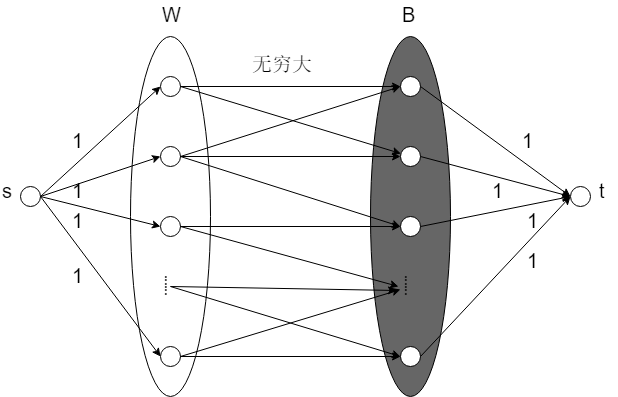
\includegraphics[scale=0.6]{image/networkflow4.png}
	\caption{骨牌问题建模}\label{fig:networkflow-tiling}
\end{figure}

\paragraph*{问题建模:}
沿用之前的处理方法,黑白相间地将棋盘做上标记,
这样棋盘的方格会被分为两个集合\((B,W)\)。
若\(|B|\)不等于\(|W|\),我们可以得出否定的结论;
若\(|B|=|W|=n\),则在B和W集之间,相邻的方格连上边,容量正无穷,
这样一来, (B,W) 相当于二分匹配中的\((V_l,\,V_r)\),
就相当于解决一个最大二分匹配问题,建模如\autoref{fig:networkflow-tiling}。

求得最大流\(f=n\),则表示该棋盘可以用骨牌填满。
\begin{itemize}
	\item 算法复杂度分析:F-F算法复杂度为\(O(mC)\),在这个模型中,m=n,\(C \le 4n\),所以用网络流解决棋盘问题的算法时间复杂度为\(O(n^2)\)。
\end{itemize}

\section{棒球比赛}
\begin{figure}[htb]
	\centering
	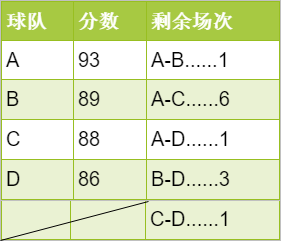
\includegraphics[scale=0.6]{image/networkflow5.png}
	\caption{棒球问题说明}\label{fig:networkflow-baseball}
\end{figure}
\begin{example}
	有四个棒球队比赛,目前赛场上的得分情况及剩余的场次如\autoref{fig:networkflow-baseball},
	问B队有没有机会赢得比赛(并列第一也算赢)?
\end{example}

\begin{figure}[h]
	\centering
	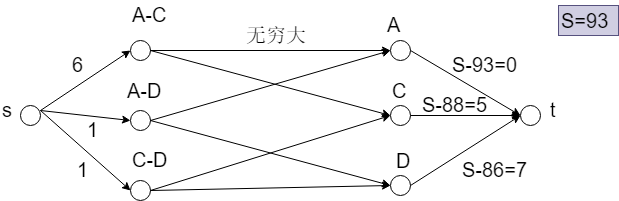
\includegraphics[scale=0.6]{image/networkflow6.png}
	\caption{棒球问题建模}\label{fig:networkflow-baseball2}
\end{figure}

\paragraph*{问题建模:}先计算若B队赢得了剩下所有可赢得的分后的总得分S。
称参赛双方相同的比赛为一类比赛。将每类比赛作为顶点,通过容量为该类比赛剩余场数的入边交于源点s,
出边指向参赛队伍,容量为正无穷;参赛队伍出边指向汇点t,容量为S-(该队伍的当前得分)。
如\autoref{fig:networkflow-baseball2}所示。

求得最大流\(f = C_{in}(t)\) ,\(C_{in}(t)\)即t的流入边容量之和,则表示B有机会赢。

\begin{figure}[htb]
	\centering
	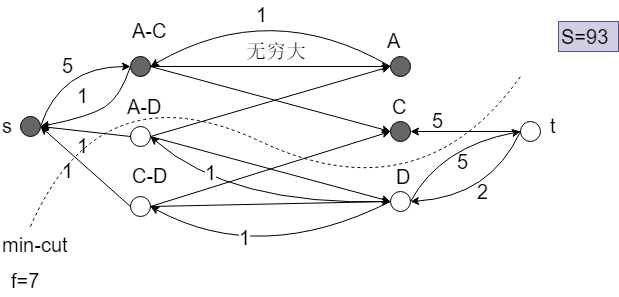
\includegraphics[scale=0.6]{image/networkflow7.png}
	\caption{棒球问题残差图}\label{fig:networkflow-baseball-reduc}
\end{figure}

\begin{itemize}
	\item 用F-F算法求模型的最大流和最小割,残差图如\autoref{fig:networkflow-baseball-reduc}。
\end{itemize}
\begin{example}
	如果初始状态,B的得分为90,那么B能否获胜?(B有机会获胜)
\end{example}

\section{项目选择问题}
\begin{example}
	有一项目的集合\{1,2,……,n\},项目之间有一定相互制约关系,完成每个项目都有一个价值\(v_i\),\(v_i\)可正可负。现要求一子集A,使得总价值p最大,且A中任一项目的前驱任务(完成一项目之前所必须完成的项目)也必须在A中。
\end{example}

\begin{figure}[htb]
	\centering
	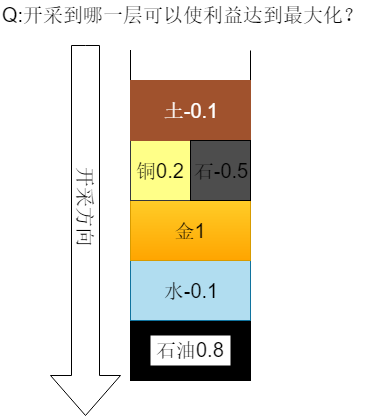
\includegraphics[scale=0.6]{image/networkflow8.png}
	\caption{项目选择示例}\label{fig:networkflow-project-select-example}
\end{figure}
为更好地理解问题,给出一更加具体地例子,如\autoref{fig:networkflow-project-select-example}所示。
\begin{figure}[htb]
	\centering
	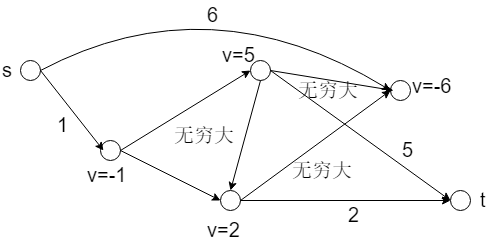
\includegraphics[scale=0.6]{image/networkflow9.png}
	\caption{项目选择建模}\label{fig:networkflow-project-select-modeling}
\end{figure}

\paragraph*{问题建模:}由于有先后的制约关系,所以原图应为一个有向图,在此基础上,引入源点s,
指向所有价值为负的项目,容量为该项目价值的绝对值;所有价值为正的项目指向汇点t,
容量为该项目的价值。对一实例的建模如\autoref{fig:networkflow-project-select-modeling}。

\begin{figure}[htb]
	\centering
	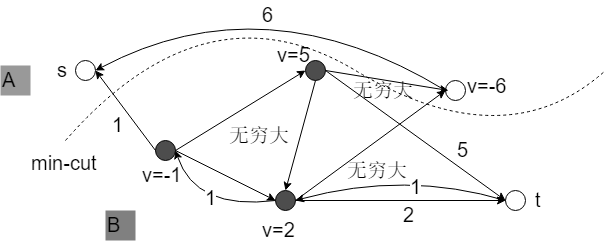
\includegraphics[scale=0.6]{image/networkflow10.png}
	\caption{项目选择问题解决}\label{fig:networkflow-project-select-solve}
\end{figure}

\begin{itemize}
	\item 用F-F算法求模型的最大流和最小割,残差图如\autoref{fig:networkflow-project-select-solve}所示,
	      其中最小割中的集合B所包含的项目即为问题的解。
\end{itemize}

\paragraph*{结果正确性分析:}
\begin{figure}[htb]
	\centering
	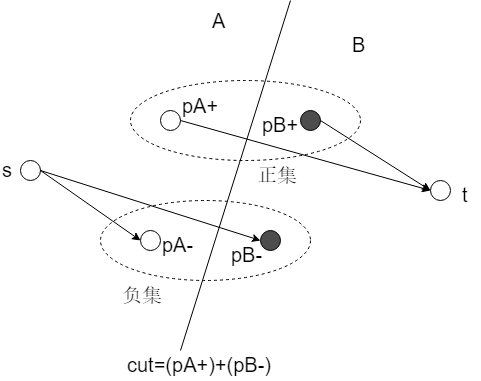
\includegraphics[scale=0.6]{image/networkflow11.png}
	\caption{项目选择问题一般情形}\label{fig:networkflow-project-select-general}
\end{figure}

\begin{itemize}
	\item 解的可行性:该模型s的所有出边容量为有限值,最坏的情况就是所有负价值点都被选入,此时最小割为s所有出边,因此最小割是包含不到无穷大的边的,此解法也就是可行的。
	\item 解为最优解:如\autoref{fig:networkflow-project-select-general}为此模型获得的一般割情形。
\end{itemize}
从\autoref{fig:networkflow-project-select-general}可求此结果的价值:
\begin{equation}
	v = (p_{B+}) - (p_{B-}) = (p_+) - (p_{A+}) - (p_{B-}) = (p_+) - [(p_{A+}) + (p_{B-})] = (p_+) - cut\\
\end{equation}
所以所得价值为一常数减去割,要求\(maxv\),则割要为\(mincut\),即\(maxv = (p_+) -mincut\)
